\chapter{Discussion of Results}

\section{Verification Methodology}

The platform was deployed locally using Docker Compose on a developer workstation, with all five services and the Kafka and PostgreSQL containers running on the same host. Each functional capability described in Chapter~4 was exercised through the web frontend, and the corresponding internal state, including database rows, Kafka topic offsets and service log lines, was inspected to verify correctness. In addition to the positive functional tests, two simulated failure scenarios were carried out: the processor service was stopped while webhooks continued to arrive, and the worker service was crashed mid-execution in order to confirm that no events were lost and that re-delivery semantics held.

\section{Functional Results}

The functional outcomes of these tests are summarised in Table~\ref{tab:results}. All ten of the scenarios that were executed produced the expected outcome, confirming that the platform meets the functional and non-functional requirements set out in Chapter~3.

\begin{table}[h]
\centering
\caption{Functional verification results.}
\label{tab:results}
\renewcommand{\arraystretch}{1.3}
\begin{tabular}{|p{6.0cm}|p{2.0cm}|p{5.0cm}|}
\hline
\textbf{Test scenario} & \textbf{Outcome} & \textbf{Observation} \\ \hline
User signup with valid input & Pass & New \texttt{User} row created, password stored as a bcrypt hash. \\ \hline
User signin with valid credentials & Pass & JWT issued; subsequent authenticated requests accepted. \\ \hline
User signin with invalid credentials & Pass & Request rejected with HTTP 403. \\ \hline
Creation of a Zap with one trigger and two actions & Pass & \texttt{Zap}, \texttt{Trigger} and two \texttt{Action} rows persisted in a single transaction. \\ \hline
Webhook invocation on the public URL & Pass & \texttt{ZapRun} and \texttt{ZapRunOutbox} rows inserted atomically. \\ \hline
Processor pickup of a new outbox row & Pass & Row read, message published to Kafka, row deleted within the next polling interval. \\ \hline
Worker execution of an email action & Pass & Email delivered to the recipient with placeholders correctly substituted. \\ \hline
Worker execution of a chained second action & Pass & Follow-up Kafka message produced and consumed; second action executed in order. \\ \hline
Webhook arrival while processor is offline & Pass & Outbox rows accumulated; on restart, the rows were processed and no events were lost. \\ \hline
Worker crash mid-execution & Pass & On restart, the un-acknowledged Kafka message was re-delivered and the action was re-executed. \\ \hline
\end{tabular}
\end{table}

Figure~\ref{fig:result-email} shows direct end-to-end evidence of the platform's correctness: a transactional email produced by the worker's \texttt{email} action and delivered to the recipient's mailbox after the corresponding Zap was fired by a webhook.

\begin{figure}[h]
\centering
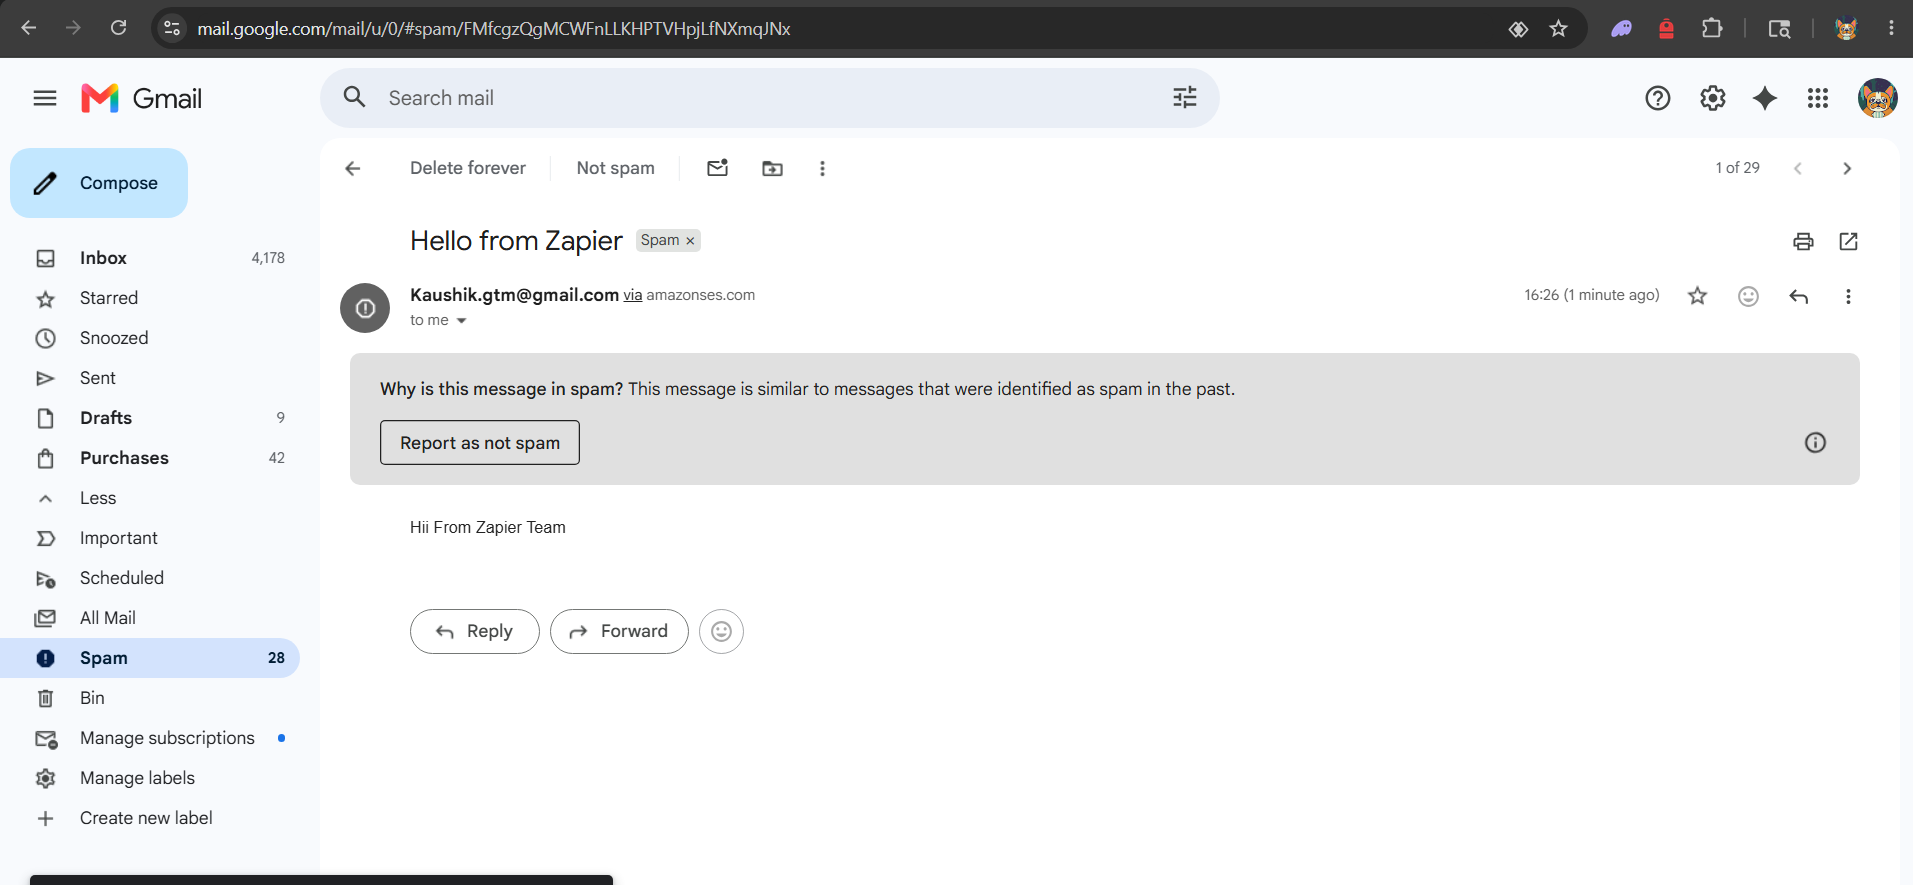
\includegraphics[width=0.95\textwidth]{figures/result-email-delivered.png}
\caption{End-to-end verification of the \texttt{email} action: a message produced by the worker, relayed over SMTP through the configured transactional-email provider, and received in the recipient's Gmail inbox. The full path exercised here is hook $\rightarrow$ outbox $\rightarrow$ processor $\rightarrow$ Kafka $\rightarrow$ worker $\rightarrow$ SMTP. The ``Why is this message in spam?'' banner is Gmail's automated heuristic for unverified senders and does not affect delivery.}
\label{fig:result-email}
\end{figure}

\section{Qualitative Observations}

\subsection{Latency}

End-to-end latency from webhook reception to first-action execution, measured informally with timestamped log lines on the development workstation, was consistently below two seconds. The dominant contributor to this latency was the processor's polling interval, which had been deliberately set to two seconds in order to keep the processor's load on the database low. Reducing this interval would lower the observed latency proportionally, at the cost of additional database queries even when the outbox table is empty.

\subsection{Throughput}

The throughput of the system was not stress-tested at scale, but the architecture imposes no inherent bottleneck other than the database itself. The worker can be scaled horizontally by adding more consumer-group members; Kafka automatically rebalances partitions across the new instances. The processor can be partitioned in the same way by sharding the outbox table or by running multiple processor instances configured to handle different ranges of the outbox primary key. Both the API and the hook services are stateless and can be replicated behind a load balancer.

\subsection{Reliability}

The two simulated failure scenarios in Table~\ref{tab:results} are the most important qualitative outcomes. They demonstrate that the transactional outbox pattern, together with manual Kafka offset commits in the worker, gives the platform the at-least-once delivery semantics specified in the non-functional requirements. In no test did a webhook event acknowledged with HTTP 200 fail to result in the eventual execution of its associated actions.

\subsection{Developer Experience}

A secondary but important outcome was the developer experience of the system. The whole platform comes up with a single \texttt{docker compose up} command, and the modular separation between services means that an engineer working on, for example, the worker can restart only that one container without affecting the rest. The use of TypeScript across the entire codebase eliminated an entire class of bugs related to property-name typos and mismatched payload shapes during integration testing.

\section{Comparison with Stated Requirements}

Table~\ref{tab:req-compliance} maps each requirement from Chapter~3 to the corresponding test scenario or implementation evidence that satisfies it. Every requirement listed is fully satisfied by the present implementation.

\begin{table}[h]
\centering
\caption{Mapping of requirements to verification evidence.}
\label{tab:req-compliance}
\renewcommand{\arraystretch}{1.3}
\begin{tabular}{|p{2.0cm}|p{6.0cm}|p{5.5cm}|}
\hline
\textbf{Req.\ ID} & \textbf{Requirement (abridged)} & \textbf{Evidence} \\ \hline
FR-1 & User signup and authentication & Tests rows 1--3, Table~\ref{tab:results} \\ \hline
FR-3 & CRUD on Zaps & Test row 4, Table~\ref{tab:results} \\ \hline
FR-4 & Unique webhook URL per Zap & Hook route \texttt{/hooks/catch/:userId/:zapId} \\ \hline
FR-5 & Actions execute in order & Test row 8, Table~\ref{tab:results} \\ \hline
FR-6 & Email and Solana actions & Worker action types, Ch.\ 4, Table 4.3 \\ \hline
FR-7 & Template substitution & Email test row 7, Table~\ref{tab:results} \\ \hline
NFR-1 & Durability across broker outages & Test row 9, Table~\ref{tab:results} \\ \hline
NFR-2 & At-least-once execution & Test row 10, Table~\ref{tab:results} \\ \hline
NFR-3 & Ordered execution & Test row 8, Table~\ref{tab:results} \\ \hline
NFR-4 & Horizontal scalability & Kafka consumer group, Ch.\ 4, \S Worker \\ \hline
NFR-6 & Single-command local startup & \texttt{docker compose up} \\ \hline
NFR-7 & Password hashing and JWT auth & Test rows 1--3, Table~\ref{tab:results} \\ \hline
\end{tabular}
\end{table}
